\documentclass[a4paper]{article}
\usepackage[utf8]{inputenc}
\usepackage[margin=0.75in]{geometry}
\usepackage{graphicx}
\usepackage{amsmath}
\usepackage{enumerate} % Import the enumerate package
\usepackage{amsfonts}
\usepackage{hyperref}
\usepackage{float}
\usepackage{listings}
\usepackage{xcolor}
\usepackage{verbatim}


% Listings settings for Python code
\lstset{
    language=Python,
    basicstyle=\ttfamily\small,
    keywordstyle=\color{blue}\bfseries,
    stringstyle=\color{red},
    commentstyle=\color{green!70!black},
    numberstyle=\tiny\color{gray},
    numbers=left,
    stepnumber=1,
    numbersep=8pt,
    showspaces=false,
    showstringspaces=false,
    frame=single,
    breaklines=true,
    breakatwhitespace=true,
    tabsize=4,
    captionpos=b
}

\title{Emergency Response: A Multi-Agent System}
\author{Sheena Maria Lang, Antonio Lobo Santos, Zachary Parent, \\ María del Carmen Ramírez Trujillo and Bruno Sánchez Gómez}
\date{\today}

\begin{document}

\maketitle
\tableofcontents
\newpage

\section{Introduction}
This report presents the final implementation and results of our multi-agent system (MAS) for emergency response coordination. Building upon our previous designs from Tasks 1 and 2, we have developed a complete, functional system that demonstrates the effectiveness of agent-based approaches in managing complex emergency scenarios.

The system is implemented using CrewAI, a framework that enables the creation and coordination of specialized agent crews. Each crew is designed with specific responsibilities and operates through well-defined processes, ensuring efficient handling of emergency situations. The implementation includes:

\begin{itemize}
    \item \textbf{Emergency Services Crew:} Handles initial emergency assessment and coordination
    \item \textbf{Firefighter Agent Crew:} Manages firefighting resources and operations
    \item \textbf{Medical Services Crew:} Coordinates medical response and hospital resources
    \item \textbf{Public Communication Crew:} Manages public information and communication
\end{itemize}

\paragraph{Report Structure:}
\begin{itemize}
    \item Section \ref{sec:crew_design} details the design and implementation of each crew, including their process definitions and data models
    \item Section \ref{sec:crew_interaction} explains the interaction mechanisms between crews and the overall system flow
    \item Section \ref{sec:results} presents the results of system testing and validation
    \item Section \ref{sec:conclusion} concludes with insights and potential future improvements
\end{itemize}

The implementation builds upon our previous design while introducing several refinements based on practical considerations and testing results. These modifications are documented and justified throughout the report. The complete source code, along with setup instructions and required input files, is provided in the accompanying project repository.

\section{Crew Design and Implementation}
\label{sec:crew_design}

\subsection{General Design Principles}
\label{subsec:design_principles}

For each crew in our system, a corresponding Python file is used to instantiate the configuration. These configurations are structured based on CrewAI's YAML schema recommendations for crews\footnote{\url{https://docs.crewai.com/concepts/crews\#yaml-configuration-recommended}}, tasks\footnote{\url{https://docs.crewai.com/concepts/tasks\#yaml-configuration-recommended}}, and agents\footnote{\url{https://docs.crewai.com/concepts/agents\#yaml-configuration-recommended}}.

These files were generated using CrewAI CLI, a universal tool for creating configurations. The following command demonstrates how to initialize a new crew configuration:\newline
\texttt{crewai create crew my\_new\_crew}\footnote{\url{https://docs.crewai.com/concepts/cli\#1-create}}.

The Python file is structured to include the following key elements:

\begin{itemize}
    \item \textbf{Imports}: Required modules, including CrewAI components such as `Agent', `Task', `Crew', and `Process'.
    \item \textbf{Tool Instantiation}: Creation of tools for task-specific functionalities.
    \item \textbf{Agent Configuration}: Agents are defined with specific properties, including their roles, goals, delegation capabilities, verbosity, and parameters for interacting with the language model (e.g., temperature settings).
    \item \textbf{Task Configuration}: Tasks are defined with descriptions, expected outputs, dependencies, and execution modes. These configurations ensure tasks are properly structured and validated. Last task of each crew includes \texttt{output\_pydantic} to ensure that the dictionaries returned to the crew are consistent.
    \item \textbf{Schema Augmentation}: Pydantic schemas can be added to the expected output of tasks using utility functions such as \texttt{add\_schema\_to\_task\_config}. This function modifies the task configuration by appending the schema JSON to the expected output property, ensuring that the LLM can take it into account.
    \item \textbf{Crew Composition}: The crew integrates agents and tasks into a defined process, executed sequentially, to accomplish its objectives.
\end{itemize}


The YAML configurations for agents and tasks specify several general properties:

\paragraph{Agent Configuration:} Agents are defined using YAML properties to specify:
\begin{itemize}
    \item \textbf{Role:} The role the agent plays within the crew.
    \item \textbf{Goal:} The overarching objective or mission assigned to the agent.
    \item \textbf{Delegation Capabilities:} Whether the agent is allowed to delegate tasks.
    \item \textbf{Language Model Parameters:} Specific settings such as the model used and the temperature to control the randomness of the output.
\end{itemize}

\paragraph{Task Configuration:} Tasks are defined in YAML with properties that include:
\begin{itemize}
    \item \textbf{Description:} A clear explanation of the purpose and workflow of the task.
    \item \textbf{Expected Output:} The structure and format of the task output, often validated against a schema.
    \item \textbf{Dependencies:} Other tasks that provide context for the task.
    \item \textbf{Execution Mode:} Specifies whether the task is executed synchronously or asynchronously (e.g., `async\_execution: true`).
\end{itemize}

This modular and schema-driven approach ensures flexibility, reusability, and validation throughout the configuration process.



\section{Crew Design and Implementation}
\label{sec:crew_design}
A design overview of the system.

\subsection{Emergency Services Crew}
\subsection{Emergency Services Crew}

The Emergency Services Crew follows a structured \textbf{sequential process} to ensure prompt handling of emergency calls and
 effective communication with response units. The crew consists of two agents: the \textbf{Emergency Call Agent} and the 
 \textbf{Notification Agent}. Each task is assigned based on the specific role and capabilities of these agents, as indicated in the 
 subsequent description.

\begin{enumerate}
    \item \textbf{Receive and Assess Call.} The \textit{Emergency Call Agent} receives incoming calls and collects relevant details
     about the incident. The information that this agent receives is the answer of the following six questions, and it saves the information
     in a report.
     \begin{itemize}
        \item Is it an indoor or outdoor fire? The answer will be outdoor or indoor.
        \item Where is it? The location is received as coordinates (x,y).
        \item Is anyone inside or trapped? The answer will be an integer number $M$ with the number of trapped people. If $M>0$, then rescues are needed and 
        the \textit{Notification Agent} will detail that to the Fire Fighters Crew.
        \item Are there hazards? The answer will be a boolean: True (yes) or False (no). Examples of hazards could be gas cylinders, 
        chemicals, explosions, etc.
        \item How big is the fire? The fire will be classified as either large (e.g. spreading rapidly), medium (e.g. smoke visible) or 
        small (e.g. small flame), depending on the assess of the \textit{Emergency Call Agent.}
        \item Is anyone injured? How badly? The answer will be a tuple with an integer number $N$ representing the number of injured 
        people and another tuple with the level of risk of each person. They could be classified based on their injuries as 'high risk',
         'risk', or 'out of risk'. If there is no victims then $N=0$ and the second element of the tuple will be an empty list.
    \end{itemize}
    
    \item \textbf{Assign fire priority level.} The \textit{Emergency Call Agent} categorizes the incident and sends initial notifications 
    to the \textit{Notification Agent}. The emergency can be classified in one of the following levels: 
    \begin{itemize}
        \item \textbf{Classifying the Fire Based on the Answers:}  
        The fire is classified into three levels based on the answers:
        \begin{itemize}
            \item \textbf{High Priority:}
            \begin{itemize}
                \item Indoor fire or outdoor fire with significant hazards (e.g., chemicals, gas).
                \item $M > 0$ (people are trapped inside).
                \item Large fire spreading rapidly.
                \item High risk injuries or multiple victims.
            \end{itemize}
            The reason of that is because a fire that is indoors, spreading quickly, with trapped people and significant hazards, 
            is clearly high priority. This combination requires an immediate and large response to prevent further harm or fatalities.
            
        \item \textbf{Medium Priority:}
            \begin{itemize}
                \item Outdoor fire with no hazards or small to medium size fire.
                \item No trapped people, but some people at risk or with moderate injuries.
                \item Medium risk injuries or a small number of victims with manageable injuries.
            \end{itemize}
            It was consider that fires that are moderately dangerous, but not life-threatening, or where injuries are serious but
             not critical, would fall into medium priority. These need quick response, but they don't have the same urgency as a high 
             priority fire.
            
        \item \textbf{Low Priority:}
            \begin{itemize}
                \item Outdoor fire with no hazards and small size.
                \item No trapped people or minimal injuries.
                \item Low risk injuries (minor burns or cuts).
            \end{itemize}
            This fire is less dangerous, with no immediate risk to life or property. A single fire engine may be enough to contain 
            and manage the situation. The priority level is low because the fire does not pose significant harm to anyone involved.
    \end{itemize}

    \item \textbf{Notify other crews.} The \textit{Notification Agent} receives the report and the classification of the fire, and 
    details the information to the appropriate crews, Medical Services Crew and Fire Fighters Crew.
    \begin{itemize}
        \item The following information is provided to the Fire Fighters:
        \begin{itemize}
            \item Location (x,y)
            \item Priority level (low, medium or high).
            \item Number of trapped people $M$.
        \end{itemize}
        \item Regarding the Medical Services, they receive the following information:
        \begin{itemize}
            \item Location (x,y)
            \item Number of injured people $N$.
            \item A list containing the risk of each injured person (out of risk, risk or high risk).
        \end{itemize}
    \end{itemize}
\end{enumerate}

\textbf{Task Dependencies} The Emergency Services Crew operates with interdependent tasks that follow a strict 
\textbf{sequential process}:
\begin{itemize}
    \item \textbf{Assign fire priority level} depends on the completion of \textbf{Receive and Assess Call}.
    \item \textbf{Notify other crews.} depends on the completion of \textbf{Categorize and Notify Response Units}.
\end{itemize}

%\begin{figure}[h]
%    \centering
%    \includegraphics[width=\textwidth]{emergency_services_flow.pdf}
%    \caption{Sequential Process Flow of the Emergency Services Crew with Agent Responsibilities}
%\end{figure}

\subsection{Emergency Services Crew}

The Emergency Services Crew follows a structured \textbf{sequential process} to ensure prompt handling of emergency calls and
 effective communication with response units. The crew consists of two agents: the \textbf{Emergency Call Agent} and the 
 \textbf{Notification Agent}. Each task is assigned based on the specific role and capabilities of these agents, as indicated in the 
 subsequent description.

\begin{enumerate}
    \item \textbf{Receive and Assess Call.} The \textit{Emergency Call Agent} receives incoming calls and collects relevant details
     about the incident. The information that this agent receives is the answer of the following six questions, and it saves the information
     in a report.
     \begin{itemize}
        \item Is it an indoor or outdoor fire? The answer will be outdoor or indoor.
        \item Where is it? The location is received as coordinates (x,y).
        \item Is anyone inside or trapped? The answer will be an integer number $M$ with the number of trapped people. If $M>0$, then rescues are needed and 
        the \textit{Notification Agent} will detail that to the Fire Fighters Crew.
        \item Are there hazards? The answer will be a boolean: True (yes) or False (no). Examples of hazards could be gas cylinders, 
        chemicals, explosions, etc.
        \item How big is the fire? The fire will be classified as either large (e.g. spreading rapidly), medium (e.g. smoke visible) or 
        small (e.g. small flame), depending on the assess of the \textit{Emergency Call Agent.}
        \item Is anyone injured? How badly? The answer will be a tuple with an integer number $N$ representing the number of injured 
        people and another tuple with the level of risk of each person. They could be classified based on their injuries as 'high risk',
         'risk', or 'out of risk'. If there is no victims then $N=0$ and the second element of the tuple will be an empty list.
    \end{itemize}
    
    \item \textbf{Assign fire priority level.} The \textit{Emergency Call Agent} categorizes the incident and sends initial notifications 
    to the \textit{Notification Agent}. The emergency can be classified in one of the following levels: 
    \begin{itemize}
        \item \textbf{Classifying the Fire Based on the Answers:}  
        The fire is classified into three levels based on the answers:
        \begin{itemize}
            \item \textbf{High Priority:}
            \begin{itemize}
                \item Indoor fire or outdoor fire with significant hazards (e.g., chemicals, gas).
                \item $M > 0$ (people are trapped inside).
                \item Large fire spreading rapidly.
                \item High risk injuries or multiple victims.
            \end{itemize}
            The reason of that is because a fire that is indoors, spreading quickly, with trapped people and significant hazards, 
            is clearly high priority. This combination requires an immediate and large response to prevent further harm or fatalities.
            
        \item \textbf{Medium Priority:}
            \begin{itemize}
                \item Outdoor fire with no hazards or small to medium size fire.
                \item No trapped people, but some people at risk or with moderate injuries.
                \item Medium risk injuries or a small number of victims with manageable injuries.
            \end{itemize}
            It was consider that fires that are moderately dangerous, but not life-threatening, or where injuries are serious but
             not critical, would fall into medium priority. These need quick response, but they don't have the same urgency as a high 
             priority fire.
            
        \item \textbf{Low Priority:}
            \begin{itemize}
                \item Outdoor fire with no hazards and small size.
                \item No trapped people or minimal injuries.
                \item Low risk injuries (minor burns or cuts).
            \end{itemize}
            This fire is less dangerous, with no immediate risk to life or property. A single fire engine may be enough to contain 
            and manage the situation. The priority level is low because the fire does not pose significant harm to anyone involved.
    \end{itemize}

    \item \textbf{Notify other crews.} The \textit{Notification Agent} receives the report and the classification of the fire, and 
    details the information to the appropriate crews, Medical Services Crew and Fire Fighters Crew.
    \begin{itemize}
        \item The following information is provided to the Fire Fighters:
        \begin{itemize}
            \item Location (x,y)
            \item Priority level (low, medium or high).
            \item Number of trapped people $M$.
        \end{itemize}
        \item Regarding the Medical Services, they receive the following information:
        \begin{itemize}
            \item Location (x,y)
            \item Number of injured people $N$.
            \item A list containing the risk of each injured person (out of risk, risk or high risk).
        \end{itemize}
    \end{itemize}
\end{enumerate}

\textbf{Task Dependencies} The Emergency Services Crew operates with interdependent tasks that follow a strict 
\textbf{sequential process}:
\begin{itemize}
    \item \textbf{Assign fire priority level} depends on the completion of \textbf{Receive and Assess Call}.
    \item \textbf{Notify other crews.} depends on the completion of \textbf{Categorize and Notify Response Units}.
\end{itemize}

%\begin{figure}[h]
%    \centering
%    \includegraphics[width=\textwidth]{emergency_services_flow.pdf}
%    \caption{Sequential Process Flow of the Emergency Services Crew with Agent Responsibilities}
%\end{figure}


\subsection{Firefighter Agent Crew}
\subsubsection{Implementation}

\paragraph{Fire Chief Agent}
The \texttt{fire\_chief} agent uses the configuration specified in \newline \texttt{self.agents\_config["fire\_chief"]}. This agent facilitates communication and coordination within the Firefighter Agent Crew and ensures the team operates effectively during emergencies.

\begin{lstlisting}[language=Python]
@agent
def fire_chief(self) -> Agent:
    return Agent(config=self.agents_config["fire_chief"])
\end{lstlisting}

\paragraph{Equipment Technician Agent}
The \texttt{equipment\_technician} agent leverages the configuration from \newline \texttt{self.agents\_config["equipment\_technician"]} to manage firefighting resources effectively by determining, packing, and maintaining necessary materials.

\begin{lstlisting}[language=Python]
@agent
def equipment_technician(self) -> Agent:
    return Agent(config=self.agents_config["equipment_technician"])
\end{lstlisting}

\paragraph{Firefighter Agent}
The \texttt{firefighter} agent is configured through \newline \texttt{self.agents\_config["firefighter"]} to deploy to fire scenes, strategize effective firefighting approaches, and ensure safety during operations.

\begin{lstlisting}[language=Python]
@agent
def firefighter(self) -> Agent:
    return Agent(config=self.agents_config["firefighter"])
\end{lstlisting}

\paragraph{Allocate Firefighting Resources Task}
This task determines the necessary firefighting materials based on the Fire Assessment, \texttt{\{fire\_assessment\}}.

\begin{lstlisting}[language=Python]
@task
def allocate_firefighting_resources(self) -> Task:
    config = add_schema_to_task_config(
        self.tasks_config["allocate_firefighting_resources"],
        FireResources.model_json_schema()
    )
    return Task(config=config, agent="equipment_technician")
\end{lstlisting}

\paragraph{Deploy Fire Combatants Task}
This task plans and executes the deployment of firefighters to the fire location, based on the Fire Assessment, \texttt{\{fire\_assessment\}}, and the resource allocation.

\begin{lstlisting}[language=Python]
@task
def deploy_fire_combatants(self) -> Task:
    config = add_schema_to_task_config(
        self.tasks_config["deploy_fire_combatants"],
        FireDeployment.model_json_schema()
    )
    return Task(config=config, agent="firefighter", context=["allocate_firefighting_resources"])
\end{lstlisting}

\paragraph{Report Firefighting Response Task}
The \texttt{report\_firefighting\_response} task provides a comprehensive summary of the firefighting response and actions taken.

\begin{lstlisting}[language=Python]
@task
def report_firefighting_response(self) -> Task:
    config = add_schema_to_task_config(
        self.tasks_config["report_firefighting_response"],
        FireResponseReport.model_json_schema()
    )
    return Task(config=config, agent="fire_chief", context=["deploy_fire_combatants"])
\end{lstlisting}

\paragraph{Crew Construction}
The Firefighter Agent Crew is constructed as a sequential process to cohesively manage tasks and agents.

\begin{lstlisting}[language=Python]
@crew
def crew(self) -> Crew:
    """Creates the Firefighter Agent Crew"""
    return Crew(
        agents=self.agents, tasks=self.tasks, process=Process.sequential, verbose=True
    )
\end{lstlisting}

\subsubsection{Implementation}

\paragraph{Fire Chief Agent}
The \texttt{fire\_chief} agent uses the configuration specified in \newline \texttt{self.agents\_config["fire\_chief"]}. This agent facilitates communication and coordination within the Firefighter Agent Crew and ensures the team operates effectively during emergencies.

\begin{lstlisting}[language=Python]
@agent
def fire_chief(self) -> Agent:
    return Agent(config=self.agents_config["fire_chief"])
\end{lstlisting}

\paragraph{Equipment Technician Agent}
The \texttt{equipment\_technician} agent leverages the configuration from \newline \texttt{self.agents\_config["equipment\_technician"]} to manage firefighting resources effectively by determining, packing, and maintaining necessary materials.

\begin{lstlisting}[language=Python]
@agent
def equipment_technician(self) -> Agent:
    return Agent(config=self.agents_config["equipment_technician"])
\end{lstlisting}

\paragraph{Firefighter Agent}
The \texttt{firefighter} agent is configured through \newline \texttt{self.agents\_config["firefighter"]} to deploy to fire scenes, strategize effective firefighting approaches, and ensure safety during operations.

\begin{lstlisting}[language=Python]
@agent
def firefighter(self) -> Agent:
    return Agent(config=self.agents_config["firefighter"])
\end{lstlisting}

\paragraph{Allocate Firefighting Resources Task}
This task determines the necessary firefighting materials based on the Fire Assessment, \texttt{\{fire\_assessment\}}.

\begin{lstlisting}[language=Python]
@task
def allocate_firefighting_resources(self) -> Task:
    config = add_schema_to_task_config(
        self.tasks_config["allocate_firefighting_resources"],
        FireResources.model_json_schema()
    )
    return Task(config=config, agent="equipment_technician")
\end{lstlisting}

\paragraph{Deploy Fire Combatants Task}
This task plans and executes the deployment of firefighters to the fire location, based on the Fire Assessment, \texttt{\{fire\_assessment\}}, and the resource allocation.

\begin{lstlisting}[language=Python]
@task
def deploy_fire_combatants(self) -> Task:
    config = add_schema_to_task_config(
        self.tasks_config["deploy_fire_combatants"],
        FireDeployment.model_json_schema()
    )
    return Task(config=config, agent="firefighter", context=["allocate_firefighting_resources"])
\end{lstlisting}

\paragraph{Report Firefighting Response Task}
The \texttt{report\_firefighting\_response} task provides a comprehensive summary of the firefighting response and actions taken.

\begin{lstlisting}[language=Python]
@task
def report_firefighting_response(self) -> Task:
    config = add_schema_to_task_config(
        self.tasks_config["report_firefighting_response"],
        FireResponseReport.model_json_schema()
    )
    return Task(config=config, agent="fire_chief", context=["deploy_fire_combatants"])
\end{lstlisting}

\paragraph{Crew Construction}
The Firefighter Agent Crew is constructed as a sequential process to cohesively manage tasks and agents.

\begin{lstlisting}[language=Python]
@crew
def crew(self) -> Crew:
    """Creates the Firefighter Agent Crew"""
    return Crew(
        agents=self.agents, tasks=self.tasks, process=Process.sequential, verbose=True
    )
\end{lstlisting}


\subsection{Medical Services Crew}
\subsubsection{Design}
\paragraph{Purpose}
The Medical Services Crew is responsible for managing and coordinating medical resources during emergency situations. This includes assessing hospital capacities, allocating resources, deploying paramedics, and ensuring timely medical response to incidents.

\paragraph{Changes}
Initially, the tasks of the Medical Services Crew were planned in a different order and with a distinct execution flow. A comparison of the initial and updated workflows is presented in \textbf{Figure} \ref{fig:exc_flow_ms_comparison}. In the updated process, the Recieve Report task was removed, since it was not necessary for the crew's operations. Additionally, the Rank Hospitals and Allocate Hospital Resources were each split into 2 separate tasks: Fetch Hospital Information and Rank Hospitals, and Plan Hospital Response and Allocate Hospital Resources, respectively. This restructuring was done to improve the efficiency and clarity of the crews' operations, since the tasks' results were poor when one agent had to perform too many steps at a time. We observed that the agents especially struggled when combining in a single task the use of a tool and the inference of logical results from said tool's output.

\begin{figure}[H]
    \centering
    \begin{subfigure}[b]{0.28\textwidth}
        \centering
        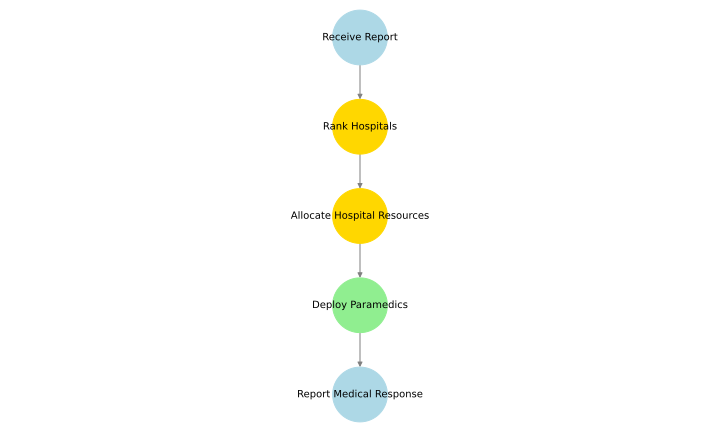
\includegraphics[width=\textwidth]{figures/Medical_Services_Crew_Flow.png}
        \caption{Initial process}
        \label{fig:initial_process}
    \end{subfigure}
    \hfill
    \begin{subfigure}[b]{0.7\textwidth}
        \centering
        \includegraphics[width=\textwidth]{figures/Medical_Services_Crew_Flow_updated.png}
        \caption{Updated process}
        \label{fig:updated_process}
    \end{subfigure}
    \caption{Comparison of the Medical Services Crew's execution flow. (a) shows the initial process, while (b) illustrates the updated process with task restructuring for improved efficiency.}
    \label{fig:exc_flow_ms_comparison}
\end{figure}

\paragraph{Structure and Components}
The Medical Services Crew leverages the \texttt{CrewBase} framework to orchestrate its agents and tasks, ensuring cohesive and efficient operations. The key components of the design are:

\begin{itemize}
    \item \textbf{Agents:}
    \begin{itemize}
        \item \texttt{medical\_services\_operator}: Facilitates communication and coordination within the Medical Services crew and with other crews, ensuring efficient information flow and timely updates during emergencies.
        \item \texttt{hospital\_coordinator}: Manages all hospitals, decides each of their responses based on proximity to emergencies, and allocates resources effectively to ensure optimal response during crises.
        \item \texttt{paramedics}: Plans the deployment of paramedics to the emergency site, including the number of paramedics, ambulances, estimated times of arrival, and any special equipment needed to handle the situation effectively.
    \end{itemize}
    \item \textbf{Tasks:}
    \begin{itemize}
        \item \texttt{fetch\_hospital\_information}: Uses the Hospital Reader Tool to fetch the information of all hospitals from the database and returns the hospital information in a structured output.
        \item \texttt{rank\_hospitals}: Receives input containing the Medical Assessment and the hospital information from the previous task, calculates the distance to the emergency location using the Route Distance Tool, and returns the list of hospital information with distances to the emergency.
        \item \texttt{plan\_hospital\_response}: Reads the ranked list of hospitals and the Medical Assessment, assesses available resources at the given hospitals, and creates an allocation plan that details how resources will be utilized to address the emergency.
        \item \texttt{allocate\_hospital\_resources}: Reads the Hospital Resource Allocation plan, uses the Hospital Updater Tool to update the database for all of the hospital resources used in the plan, and confirms that the hospital resources have been successfully allocated.
        \item \texttt{deploy\_paramedics}: Reads the Hospital Resource Allocation plan and the Medical Assessment, calculates the total number of paramedics to be deployed and ambulances to be dispatched, determines the estimated times of arrival, and identifies any special equipment required.
        \item \texttt{report\_medical\_response}: Reads the Hospital Resource Allocation plan, the Paramedic Deployment plan, and the Medical Assessment, compiles a comprehensive summary of the medical response plan, and provides a detailed report for future reference and continuous improvement.
    \end{itemize}
    \item \textbf{Crew:}
    The crew is constructed using the \texttt{Crew} class, which integrates the agents and tasks into a seamless workflow. This design ensures effective progression from hospital information retrieval and resource allocation to paramedic deployment and medical response reporting.
\end{itemize}
The modular design of the Medical Services Crew enables it to adapt to a wide range of emergency scenarios, ensuring efficient and timely medical response to incidents.


\subsubsection{Design}
\paragraph{Purpose}
The Medical Services Crew is responsible for managing and coordinating medical resources during emergency situations. This includes assessing hospital capacities, allocating resources, deploying paramedics, and ensuring timely medical response to incidents.

\paragraph{Changes}
Initially, the tasks of the Medical Services Crew were planned in a different order and with a distinct execution flow. A comparison of the initial and updated workflows is presented in \textbf{Figure} \ref{fig:exc_flow_ms_comparison}. In the updated process, the Recieve Report task was removed, since it was not necessary for the crew's operations. Additionally, the Rank Hospitals and Allocate Hospital Resources were each split into 2 separate tasks: Fetch Hospital Information and Rank Hospitals, and Plan Hospital Response and Allocate Hospital Resources, respectively. This restructuring was done to improve the efficiency and clarity of the crews' operations, since the tasks' results were poor when one agent had to perform too many steps at a time. We observed that the agents especially struggled when combining in a single task the use of a tool and the inference of logical results from said tool's output.

\begin{figure}[H]
    \centering
    \begin{subfigure}[b]{0.28\textwidth}
        \centering
        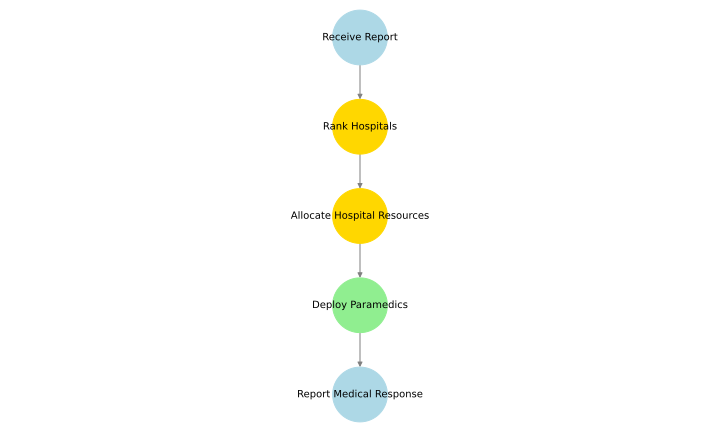
\includegraphics[width=\textwidth]{figures/Medical_Services_Crew_Flow.png}
        \caption{Initial process}
        \label{fig:initial_process}
    \end{subfigure}
    \hfill
    \begin{subfigure}[b]{0.7\textwidth}
        \centering
        \includegraphics[width=\textwidth]{figures/Medical_Services_Crew_Flow_updated.png}
        \caption{Updated process}
        \label{fig:updated_process}
    \end{subfigure}
    \caption{Comparison of the Medical Services Crew's execution flow. (a) shows the initial process, while (b) illustrates the updated process with task restructuring for improved efficiency.}
    \label{fig:exc_flow_ms_comparison}
\end{figure}

\paragraph{Structure and Components}
The Medical Services Crew leverages the \texttt{CrewBase} framework to orchestrate its agents and tasks, ensuring cohesive and efficient operations. The key components of the design are:

\begin{itemize}
    \item \textbf{Agents:}
    \begin{itemize}
        \item \texttt{medical\_services\_operator}: Facilitates communication and coordination within the Medical Services crew and with other crews, ensuring efficient information flow and timely updates during emergencies.
        \item \texttt{hospital\_coordinator}: Manages all hospitals, decides each of their responses based on proximity to emergencies, and allocates resources effectively to ensure optimal response during crises.
        \item \texttt{paramedics}: Plans the deployment of paramedics to the emergency site, including the number of paramedics, ambulances, estimated times of arrival, and any special equipment needed to handle the situation effectively.
    \end{itemize}
    \item \textbf{Tasks:}
    \begin{itemize}
        \item \texttt{fetch\_hospital\_information}: Uses the Hospital Reader Tool to fetch the information of all hospitals from the database and returns the hospital information in a structured output.
        \item \texttt{rank\_hospitals}: Receives input containing the Medical Assessment and the hospital information from the previous task, calculates the distance to the emergency location using the Route Distance Tool, and returns the list of hospital information with distances to the emergency.
        \item \texttt{plan\_hospital\_response}: Reads the ranked list of hospitals and the Medical Assessment, assesses available resources at the given hospitals, and creates an allocation plan that details how resources will be utilized to address the emergency.
        \item \texttt{allocate\_hospital\_resources}: Reads the Hospital Resource Allocation plan, uses the Hospital Updater Tool to update the database for all of the hospital resources used in the plan, and confirms that the hospital resources have been successfully allocated.
        \item \texttt{deploy\_paramedics}: Reads the Hospital Resource Allocation plan and the Medical Assessment, calculates the total number of paramedics to be deployed and ambulances to be dispatched, determines the estimated times of arrival, and identifies any special equipment required.
        \item \texttt{report\_medical\_response}: Reads the Hospital Resource Allocation plan, the Paramedic Deployment plan, and the Medical Assessment, compiles a comprehensive summary of the medical response plan, and provides a detailed report for future reference and continuous improvement.
    \end{itemize}
    \item \textbf{Crew:}
    The crew is constructed using the \texttt{Crew} class, which integrates the agents and tasks into a seamless workflow. This design ensures effective progression from hospital information retrieval and resource allocation to paramedic deployment and medical response reporting.
\end{itemize}
The modular design of the Medical Services Crew enables it to adapt to a wide range of emergency scenarios, ensuring efficient and timely medical response to incidents.



\subsection{Public Communication Crew}
\subsubsection{Implementation}

\paragraph{Communication Operator Agent}
The \texttt{communication\_operator} agent uses the configuration specified in \newline \texttt{self.agents\_config["communication\_operator"]}. This agent facilitates communication between emergency crews and public communication teams, ensuring clarity and accuracy in information flow.

\begin{lstlisting}[language=Python]
@agent
def communication_operator(self) -> Agent:
    return Agent(config=self.agents_config["communication_operator"])
\end{lstlisting}

\paragraph{Archive Keeper Agent}
The \texttt{archive\_keeper} agent leverages the configuration from \newline \texttt{self.agents\_config["archive\_keeper"]} to manage historical data archives, providing quick access to relevant past incident reports and trends.

\begin{lstlisting}[language=Python]
@agent
def archive_keeper(self) -> Agent:
    return Agent(config=self.agents_config["archive_keeper"])
\end{lstlisting}

\paragraph{Article Writer Agent}
The \texttt{article\_writer} agent is configured through \newline \texttt{self.agents\_config["article\_writer"]} to draft, refine, and integrate informative articles for public dissemination.

\begin{lstlisting}[language=Python]
@agent
def article_writer(self) -> Agent:
    return Agent(config=self.agents_config["article_writer"])
\end{lstlisting}

\paragraph{Mayor Agent}
The \texttt{mayor} agent ensures oversight by reviewing and authorizing final communications, as configured in \newline \texttt{self.agents\_config["mayor"]}.

\begin{lstlisting}[language=Python]
@agent
def mayor(self) -> Agent:
    return Agent(config=self.agents_config["mayor"])
\end{lstlisting}

\paragraph{Social Media Commentator Agent}
The \texttt{social\_media\_commentator} agent, configured via \newline \texttt{self.agents\_config["social\_media\_commentator"]}, provides witty yet constructive commentary for social media engagement.

\begin{lstlisting}[language=Python]
@agent
def social_media_commentator(self) -> Agent:
    return Agent(config=self.agents_config["social_media_commentator"])
\end{lstlisting}

\paragraph{Search Related Cases Task}
This task utilizes the \texttt{RelatedCases} model to analyze historical data and identify trends or reoccurring issues. To force the tool output as the result of an agent's task, the \texttt{result\_as\_answer} parameter is set to \texttt{True}, ensuring the tool output is captured and returned as the task result without modifications by the agent.

\begin{lstlisting}[language=Python]
@task
def search_related_cases(self) -> Task:
    config = add_schema_to_task_config(
        self.tasks_config["search_related_cases"], RelatedCases.model_json_schema()
    )
    return Task(config=config, tools=[IncidentAnalysisTool(result_as_answer=True)])
\end{lstlisting}

\paragraph{Draft Initial Article Task}
The task generates an initial draft for public dissemination based on structured incident data.

\begin{lstlisting}[language=Python]
@task
def draft_initial_article(self) -> Task:
    config = add_schema_to_task_config(
        self.tasks_config["draft_initial_article"], DraftArticle.model_json_schema()
    )
    return Task(config=config)
\end{lstlisting}

\paragraph{Integrate Additional Information Task}
This task integrates supplementary historical data and refines the article for professional publication.

\begin{lstlisting}[language=Python]
@task
def integrate_additional_information(self) -> Task:
    config = add_schema_to_task_config(
        self.tasks_config["integrate_additional_information"],
        IntegratedArticle.model_json_schema(),
    )
    return Task(config=config)
\end{lstlisting}

\paragraph{Review and Authorize Publication Task}
The \texttt{review\_and\_authorize\_publication} task ensures that communications adhere to policies and meet quality standards.

\begin{lstlisting}[language=Python]
@task
def review_and_authorize_publication(self) -> Task:
    config = add_schema_to_task_config(
        self.tasks_config["review_and_authorize_publication"],
        ReviewedArticle.model_json_schema(),
    )
    return Task(config=config)
\end{lstlisting}

\paragraph{Provide Social Media Feedback Task}
This task evaluates the public-facing content and adds a lighthearted commentary for engagement.

\begin{lstlisting}[language=Python]
@task
def provide_social_media_feedback(self) -> Task:
    return Task(config=self.tasks_config["provide_social_media_feedback"])
\end{lstlisting}

\paragraph{Publish Final Communication Task}
The final task consolidates and publishes the refined article along with mayoral approval and social media feedback.

\begin{lstlisting}[language=Python]
@task
def publish_final_communication(self) -> Task:
    config = add_schema_to_task_config(
        self.tasks_config["publish_final_communication"],
        PublicCommunicationReport.model_json_schema(),
    )
    return Task(config=config, output_pydantic=PublicCommunicationReport)
\end{lstlisting}

\paragraph{Crew Construction}
The Public Communication Crew is constructed as a sequential process to manage tasks and agents cohesively.

\begin{lstlisting}[language=Python]
@crew
def crew(self) -> Crew:
    """Creates the Public Communication Crew"""
    return Crew(
        agents=self.agents, tasks=self.tasks, process=Process.sequential, verbose=True
    )
\end{lstlisting}

\subsubsection{Implementation}

\paragraph{Communication Operator Agent}
The \texttt{communication\_operator} agent uses the configuration specified in \newline \texttt{self.agents\_config["communication\_operator"]}. This agent facilitates communication between emergency crews and public communication teams, ensuring clarity and accuracy in information flow.

\begin{lstlisting}[language=Python]
@agent
def communication_operator(self) -> Agent:
    return Agent(config=self.agents_config["communication_operator"])
\end{lstlisting}

\paragraph{Archive Keeper Agent}
The \texttt{archive\_keeper} agent leverages the configuration from \newline \texttt{self.agents\_config["archive\_keeper"]} to manage historical data archives, providing quick access to relevant past incident reports and trends.

\begin{lstlisting}[language=Python]
@agent
def archive_keeper(self) -> Agent:
    return Agent(config=self.agents_config["archive_keeper"])
\end{lstlisting}

\paragraph{Article Writer Agent}
The \texttt{article\_writer} agent is configured through \newline \texttt{self.agents\_config["article\_writer"]} to draft, refine, and integrate informative articles for public dissemination.

\begin{lstlisting}[language=Python]
@agent
def article_writer(self) -> Agent:
    return Agent(config=self.agents_config["article_writer"])
\end{lstlisting}

\paragraph{Mayor Agent}
The \texttt{mayor} agent ensures oversight by reviewing and authorizing final communications, as configured in \newline \texttt{self.agents\_config["mayor"]}.

\begin{lstlisting}[language=Python]
@agent
def mayor(self) -> Agent:
    return Agent(config=self.agents_config["mayor"])
\end{lstlisting}

\paragraph{Social Media Commentator Agent}
The \texttt{social\_media\_commentator} agent, configured via \newline \texttt{self.agents\_config["social\_media\_commentator"]}, provides witty yet constructive commentary for social media engagement.

\begin{lstlisting}[language=Python]
@agent
def social_media_commentator(self) -> Agent:
    return Agent(config=self.agents_config["social_media_commentator"])
\end{lstlisting}

\paragraph{Search Related Cases Task}
This task utilizes the \texttt{RelatedCases} model to analyze historical data and identify trends or reoccurring issues. To force the tool output as the result of an agent's task, the \texttt{result\_as\_answer} parameter is set to \texttt{True}, ensuring the tool output is captured and returned as the task result without modifications by the agent.

\begin{lstlisting}[language=Python]
@task
def search_related_cases(self) -> Task:
    config = add_schema_to_task_config(
        self.tasks_config["search_related_cases"], RelatedCases.model_json_schema()
    )
    return Task(config=config, tools=[IncidentAnalysisTool(result_as_answer=True)])
\end{lstlisting}

\paragraph{Draft Initial Article Task}
The task generates an initial draft for public dissemination based on structured incident data.

\begin{lstlisting}[language=Python]
@task
def draft_initial_article(self) -> Task:
    config = add_schema_to_task_config(
        self.tasks_config["draft_initial_article"], DraftArticle.model_json_schema()
    )
    return Task(config=config)
\end{lstlisting}

\paragraph{Integrate Additional Information Task}
This task integrates supplementary historical data and refines the article for professional publication.

\begin{lstlisting}[language=Python]
@task
def integrate_additional_information(self) -> Task:
    config = add_schema_to_task_config(
        self.tasks_config["integrate_additional_information"],
        IntegratedArticle.model_json_schema(),
    )
    return Task(config=config)
\end{lstlisting}

\paragraph{Review and Authorize Publication Task}
The \texttt{review\_and\_authorize\_publication} task ensures that communications adhere to policies and meet quality standards.

\begin{lstlisting}[language=Python]
@task
def review_and_authorize_publication(self) -> Task:
    config = add_schema_to_task_config(
        self.tasks_config["review_and_authorize_publication"],
        ReviewedArticle.model_json_schema(),
    )
    return Task(config=config)
\end{lstlisting}

\paragraph{Provide Social Media Feedback Task}
This task evaluates the public-facing content and adds a lighthearted commentary for engagement.

\begin{lstlisting}[language=Python]
@task
def provide_social_media_feedback(self) -> Task:
    return Task(config=self.tasks_config["provide_social_media_feedback"])
\end{lstlisting}

\paragraph{Publish Final Communication Task}
The final task consolidates and publishes the refined article along with mayoral approval and social media feedback.

\begin{lstlisting}[language=Python]
@task
def publish_final_communication(self) -> Task:
    config = add_schema_to_task_config(
        self.tasks_config["publish_final_communication"],
        PublicCommunicationReport.model_json_schema(),
    )
    return Task(config=config, output_pydantic=PublicCommunicationReport)
\end{lstlisting}

\paragraph{Crew Construction}
The Public Communication Crew is constructed as a sequential process to manage tasks and agents cohesively.

\begin{lstlisting}[language=Python]
@crew
def crew(self) -> Crew:
    """Creates the Public Communication Crew"""
    return Crew(
        agents=self.agents, tasks=self.tasks, process=Process.sequential, verbose=True
    )
\end{lstlisting}


\section{Crew Interactions and Flow}
\label{sec:crew_interaction}

\subsection{Design and Coordination}
The Emergency Planner Flow is designed to handle emergency situations by coordinating multiple crews. The flow begins with the retrieval of a call transcript, followed by the processing of the call by emergency services. Based on the assessment, firefighters and medical services are dispatched in parallel. Public communication is managed after both teams report or during approval retries. Once the emergency is resolved, the flow concludes with the generation of a comprehensive emergency report, which includes summaries and timestamps from all participating crews.

\subsubsection{State Management}
The system maintains a centralized state using a Pydantic model \footnote{\url{https://docs.crewai.com/concepts/flows\#structured-state-management}}, `EmergencyPlannerState`, which tracks all aspects of the emergency response. This includes the call transcript, assessments, and response reports. The state model ensures type-safe storage and accommodates partial updates.

\subsection{Implementation}
The flow is orchestrated using CrewAI's decorators, which define the sequence and conditions for crew operations. Key flow control points include:

\begin{itemize}
    \item \texttt{@start()}\footnote{\url{https://docs.crewai.com/concepts/flows\#start}} for initiating the call transcript retrieval.
    \item \texttt{@listen()}\footnote{\url{https://docs.crewai.com/concepts/flows\#listen}} for establishing dependencies between operations, such as emergency services processing and the dispatch of firefighters and medical services.
    \item \texttt{@router()}\footnote{\url{https://docs.crewai.com/concepts/flows\#router}} for handling conditional flow control, particularly for public communication approval.
\end{itemize}


\subsubsection{Router}
The router manages public communication approval, checking if the mayor has approved the communication. If not, it retries up to a maximum count. This ensures that public communication is handled appropriately and efficiently.
This includes the use of \texttt{and\_} and \texttt{or\_} to combine multiple conditions. This is key for the retry mechanism for public communication approval.

\paragraph{Complex Logic for Public Communications}
\texttt{and\_} \footnote{\url{https://docs.crewai.com/concepts/flows\#conditional-logic-and}} and \texttt{or\_} \footnote{\url{https://docs.crewai.com/concepts/flows\#conditional-logic-or}} are used to combine multiple conditions. This is key for the retry mechanism for public communication approval.

\begin{lstlisting}[language=Python]
@listen(or_(and_(firefighters, medical_services), "retry_public_communication"))
def public_communication(self):
    # ...
\end{lstlisting}

\paragraph{Router Logic for Public Communication Approval}
The router emits different messages based on the conditions, either triggering a retry or saving the full emergency report.

\begin{lstlisting}[language=Python]
@router(public_communication)
def check_approval(self):
    logger.info("Checking approval")
    if self.state.public_communication_report.mayor_approved:
        return "save full emergency report"
    elif self.state.mayor_approval_retry_count >= MAX_MAYOR_APPROVAL_RETRY_COUNT:
        return "save full emergency report"
    self.state.mayor_approval_retry_count += 1
    return "retry_public_communication"
\end{lstlisting}

\subsection{Justification of Design Choices}
The design choices are justified by the need for a robust and flexible system that can handle complex emergency scenarios. The use of CrewAI's flow decorators allows for clear and maintainable code, while the parallel processing capabilities ensure timely responses from different crews.


\section{Testing}
\label{sec:testing}

\subsection{Unit Tests}
\label{subsec:unit_tests}

The unit testing framework for evaluating different agent crews is structured to be modular and scalable, accommodating diverse agents with varying input requirements. Below, we outline the folder structure, testing script, execution process, and input configuration to ensure a comprehensive and systematic evaluation.

\subsubsection*{Folder Structure}
The directory structure of the project is as follows:

\begin{description}
    \item[\texttt{test/}] The main testing folder containing inputs, logs, and results.
    \begin{description}
        \item[\texttt{inputs/}] Contains JSON files defining the test cases, e.g., \texttt{test\_PC.json} for Public Communication Crew.
        \item[\texttt{logs/}] Stores execution logs, including \texttt{test.log} for detailed information about each test run.
        \item[\texttt{results/}] Saves the output of each test, such as \texttt{PublicCommunicationCrew\_output\_1.txt}.
    \end{description}
    \item[\texttt{test.py}] The main script responsible for loading, testing, and logging results.
\end{description}

\subsubsection*{Testing Script}
The testing script, \texttt{test.py}, is the core of the framework and is responsible for loading test cases, executing the corresponding agents, and logging the results. Key features include:

\begin{itemize}
    \item \textbf{Dynamic Crew Mapping}: The script dynamically maps crew names (e.g., \texttt{PublicCommunicationCrew}) to their respective Python classes for instantiation.
    \item \textbf{Logging}: Logs are stored in \texttt{test/logs/test.log} and include detailed information about each test case, intermediate results, and final outputs.
    \item \textbf{Input Validation}: Inputs are validated using Pydantic models from the \texttt{data\_models} package to ensure consistency and type safety.
    \item \textbf{Result Storage}: Results of each test are saved in \texttt{test/results/} with a structured format for easy review.
\end{itemize}

\subsubsection*{Execution Process}
The process for running the tests is as follows:

\begin{enumerate}
    \item \textbf{Prepare Input JSON}: Create or modify test cases in \texttt{test/inputs/}. Each JSON file should contain an array of test cases with fields specifying the crew to test and the inputs required.
    \item \textbf{Run the Script}: Execute \texttt{test.py} using Python. For example:
    \begin{verbatim}
    python test.py
    \end{verbatim}
    \item \textbf{Review Logs}: Check the log file in \texttt{test/logs/test.log} for detailed execution information.
    \item \textbf{Review Results}: Inspect output files in \texttt{test/results/} for the results of each test case.
\end{enumerate}

\subsubsection*{Input Configuration}
The inputs for testing are defined in JSON format, where each test case specifies the crew to be executed and the required inputs. Below is an example:

\begin{lstlisting}[language=json, caption={Example Input JSON for Testing Crews}]
{
    "test_cases": [
        {
            "crew_to_test": "EmergencyServicesCrew",
            "crew_inputs": {
                "transcript": "There's a small fire at 456 Elm St. People might be trapped."
            }
        },
        {
            "crew_to_test": "FirefightersCrew",
            "crew_inputs": {
                "fire_assessment": {
                    "fire_severity": 2,
                    "medical_services_required": true,
                    "location": [123.45, 678.90]
                }
            }
        }        
    ]
}
\end{lstlisting}

\subsubsection*{Advantages}
This framework offers the following advantages:

\begin{itemize}
    \item \textbf{Modular Design}: Each agent crew is implemented and tested independently, ensuring modularity and ease of debugging.
    \item \textbf{Type Safety}: Pydantic models enforce input validation, reducing runtime errors and ensuring consistent data structure.
    \item \textbf{Scalability}: New agent crews can be added by implementing their logic and updating the crew mapping in \texttt{test.py}.
    \item \textbf{Traceability}: Detailed logging captures both intermediate and final outputs, enhancing reproducibility.
\end{itemize}

This structure ensures a clear, efficient, and scientifically rigorous approach to unit testing multi-agent systems.

\subsection{Integration Tests}
\label{subsec:integration_tests}

\subsection{Results}
\label{subsec:results}



\section{Conclusion}
\label{sec:conclusion}
% This report presents a comprehensive multi-agent system for emergency response coordination, implementing sophisticated cooperation mechanisms across specialized crews. The key achievements and insights include:

% \begin{itemize}
%     \item \textbf{Process Definition:} Each crew operates with clearly defined sequential workflows:
%     \begin{itemize}
%         \item Emergency Services established structured protocols for initial assessment and crew dispatch
%         \item Firefighters implemented systematic resource allocation and deployment procedures
%         \item Medical Services developed efficient hospital ranking and resource coordination
%         \item Public Communications created an iterative approval workflow with historical case integration
%     \end{itemize}
    
%     \item \textbf{Data Standardization:} Implementation of Pydantic models ensures:
%     \begin{itemize}
%         \item Type-safe data transfer between crews
%         \item Consistent reporting formats
%         \item Structured storage of emergency response states
%     \end{itemize}
    
%     \item \textbf{Coordination Mechanisms:} The system achieves efficient crew interaction through:
%     \begin{itemize}
%         \item Centralized state management
%         \item Parallel processing capabilities
%         \item Sophisticated routing mechanisms
%         \item Retry systems for critical operations
%     \end{itemize}
% \end{itemize}

% The framework demonstrates the effectiveness of structured agent cooperation in emergency response scenarios. Future work could explore the integration of additional specialized crews (such as Forensics) and further optimization of the coordination mechanisms for larger-scale emergencies.

\section{References}
% \bibliography{references}
% \bibliographystyle{plain}
\end{document}
